\section{Ergebnisse und Fazit} \label{sec:ergebnisse}

Das gesetzte Ziel, ein kleines Roboterfahrzeug zu befähigen über CNN's frei im Raum zu fahren, ohne dabei mit Hindernissen zu kollidieren, konnte erreicht werden. Dabei wurden als Grundlage die Fragen beantwortet, was ein Convolutional neural Network (CNN) ist, wie diese aufgebaut sind und warum Transfer Learning eine gute Wahl ist, um schnell mit wenig Trainingsdaten ein Modell bezüglich bestimmter Fähigkeiten anzulernen.\\
Jedoch muss festgehalten werden, dass es nur in den meisten Fällen möglich war Kollisionen zu vermeiden. Besonders schlecht beleuchtete Umgebungen oder unbekannte Gebiete in der Wohnung sorgten für erhöhte Fehlerraten, wo Kollisionen nicht vermieden werden konnten. Das Konzept scheint also in diesem simplen Ansatz nicht auf ein realen Verkehrsteilnehmer übertragbar zu sein. Dafür müsste das Modell deutlich intensiver mit mehr Bildern aber auch mehr Klassen trainiert werden, um Situationen \bzw Szenarien besser differenzieren und einschätzen zu können.\\
Dennoch konnte nachgewiesen werden, dass es mit wenigen Zeilen Code bereits möglich ist eine fähige künstliche Intelligenz zu implementieren, die einfache Aufgaben zuverlässig umsetzen kann.

\begin{wrapfigure}{r}{0.64\textwidth}
    \centering
    \fbox{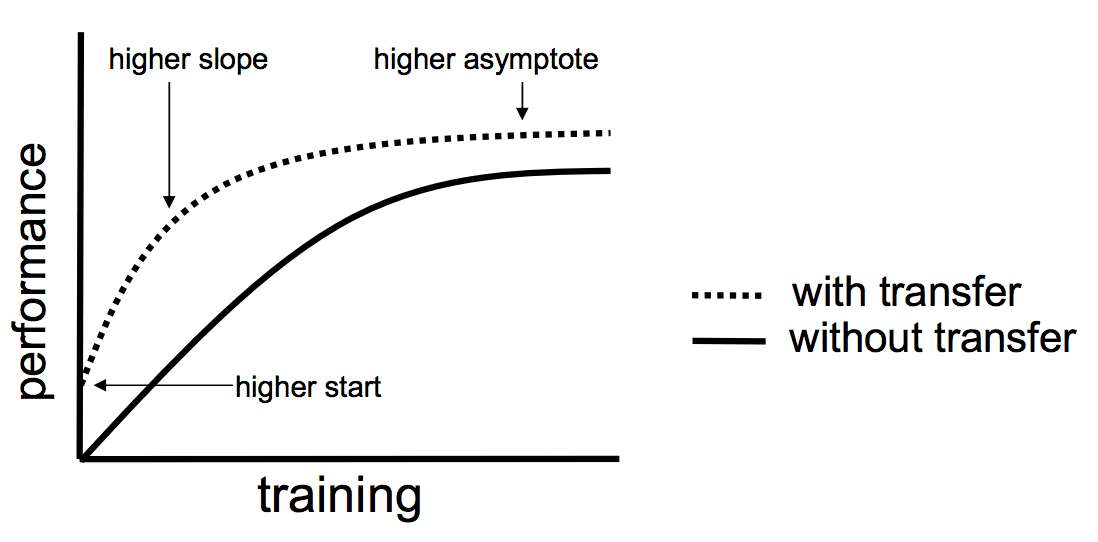
\includegraphics[width=0.62\textwidth]{Bilder/transfer-learning.png}}
    \caption[Vorteile des Transfer Learning]{Vorteile des Transfer Learning \cite{Brownlee2017}}
    \label{fig:Bild5.1}
\end{wrapfigure}

Weiterhin hat sich gezeigt, dass die Nutzung von CNN's mit mehr Layern (\zB ResNet50) dafür sorgt, dass die antrainierten Modelle akkurater werden. Jedoch erhöhen sich damit auch die Anforderungen an die Hardware, insbesondere die GPU. Es konnte festgestellt werden, dass die Reaktionszeit des Jetbots sichtbar langsamer war, desto komplexer das genutzte neuronale Netz ist. Das AlexNet hat sich als Sweetspot erwiesen mit dem gewählten Jetson Nano. Es gibts jedoch bereits heute schon sehr kompakte und deutlich effizientere Mikrocontroller (meist von Nvidia) die eine tausendfache Leistung im Vergleich zu der genutzten Hardware haben. \\
Das Pre-Training hat sich hingegen als eine kleinere Herausforderung dargestellt, da dieses auf einem separaten Computer stattfinden konnte, welcher mit einer Hochleistungsgrafikkarte (Nvidia RTX 3090) ausgestattet ist.